%% inicio, la clase del documento es iccmemoria.cls
\documentclass{smartTraining}
\usepackage{amsmath}
\usepackage{mhchem}
%\usepackage{chemfig}
\usepackage{makecell}
\renewcommand{\arraystretch}{3}
%% datos generales y para la tapa
\titulo{\textit{Smart Training}, Servicio web de Entrenamiento de Modelos}
\author{David Alfredo Medina Ortiz}
\supervisor{�lvaro Olivera Nappa, Ph.D.}
\director{Profesor del curso}
\date{Agosto, 2018}

%% inicio de documento
\begin{document}

%% crea la tapa
\maketitle

%%% dedicatoria
%\begin{dedicatory}
%Dedicado a ...
%\end{dedicatory}
%
%%% agradecimientos
%\begin{acknowledgment}
%Agradecimientos a ...
%\end{acknowledgment}

%% indices
\tableofcontents
\listoffigures
\listoftables

%% resumen
\begin{resumen}

Conceptos como miner�a de datos, machine learning, big data, an�lisis estad�sticos, modelamientos matem�ticos, etc, son mencionados d�a a d�a, ya sea en el �mbito privado como p�blico, involucrando �reas como: comercio, salud, investigaci�n, transporte, etc. Lo cual denota que son tem�ticas que han adquirido mayor relevancia y su ascenso seguir� con el pasar del tiempo.

La manipulaci�n de grandes vol�menes de datos, con el fin de poder extraer informaci�n de ellos, b�squeda de patrones, evaluaciones estad�sticas, etc. Implica por parte del interesado, tener conocimientos en dichas �reas adem�s de comprender herramientas inform�ticas que le permitan dicho procedimiento. Sin embargo, dichas herramientas o son costosas, debido a la licencia que implica, o, se requiere de conocimiento inform�tico para su manipulaci�n, debido a que requiere implementar m�dulos o servicios a medida que permitan ejecutar las tareas de inter�s, lo cual deja a un n�mero importante de entidades que desean involucrarse en dicho mundo, pero no cuentan con las capacidades ni tampoco con las competencias para ello.

Dado a lo anterior y en base a la creciente demanda de desarrollo de metodolog�as que permitan aplicar data mining a procesos de datos, con el fin de extraer informaci�n y conocimiento de la misma, se propone Smart Training, como sistema web, que facilite los procesos de evaluaciones estad�sticas, b�squeda de patrones de comportamiento, desarrollo de modelos de clasificaci�n y evaluaci�n de caracter�sticas o features en el set de datos a estudiar.

			%resumen...
\end{resumen}

\chapter{INTRODUCCI�N}

\section{Data Mining}

Miner�a de datos es el proceso de descubrimiento de patrones en set de datos, involucrando m�todos asociados a Machine Learning, Estad�sticas y sistemas de bases de datos. \cite{intro1}. La miner�a de datos es un subcampo interdisciplinario de la inform�tica, el cual tiene por objetivo general extraer informaci�n (a trav�s de m�todos inteligentes) de un conjunto de datos y transformar la informaci�n en una estructura comprensible para su uso posterior. \cite{intro2, intro3}. La miner�a de datos es el paso de an�lisis del proceso de \textit{descubrimiento de conocimiento en bases de datos}, o KDD. \cite{intro4}. Adem�s del an�lisis en bruto de los datos, tambi�n incluye aspectos de manipulaci�n de bases de datos, pre procesamiento de datos, evaluaciones de modelo e inferencia, m�tricas de inter�s, consideraciones de complejidad, post procesamiento de estructuras descubiertas, visualizaci�n y actualizaci�n de la informaci�n.

En la Figura \ref{intro1}, se exponen las principales ramas que componen la miner�a de datos y los diferentes procesos que se asocian a dichas ramas.

\begin{figure}[!h]
	
	\centering
	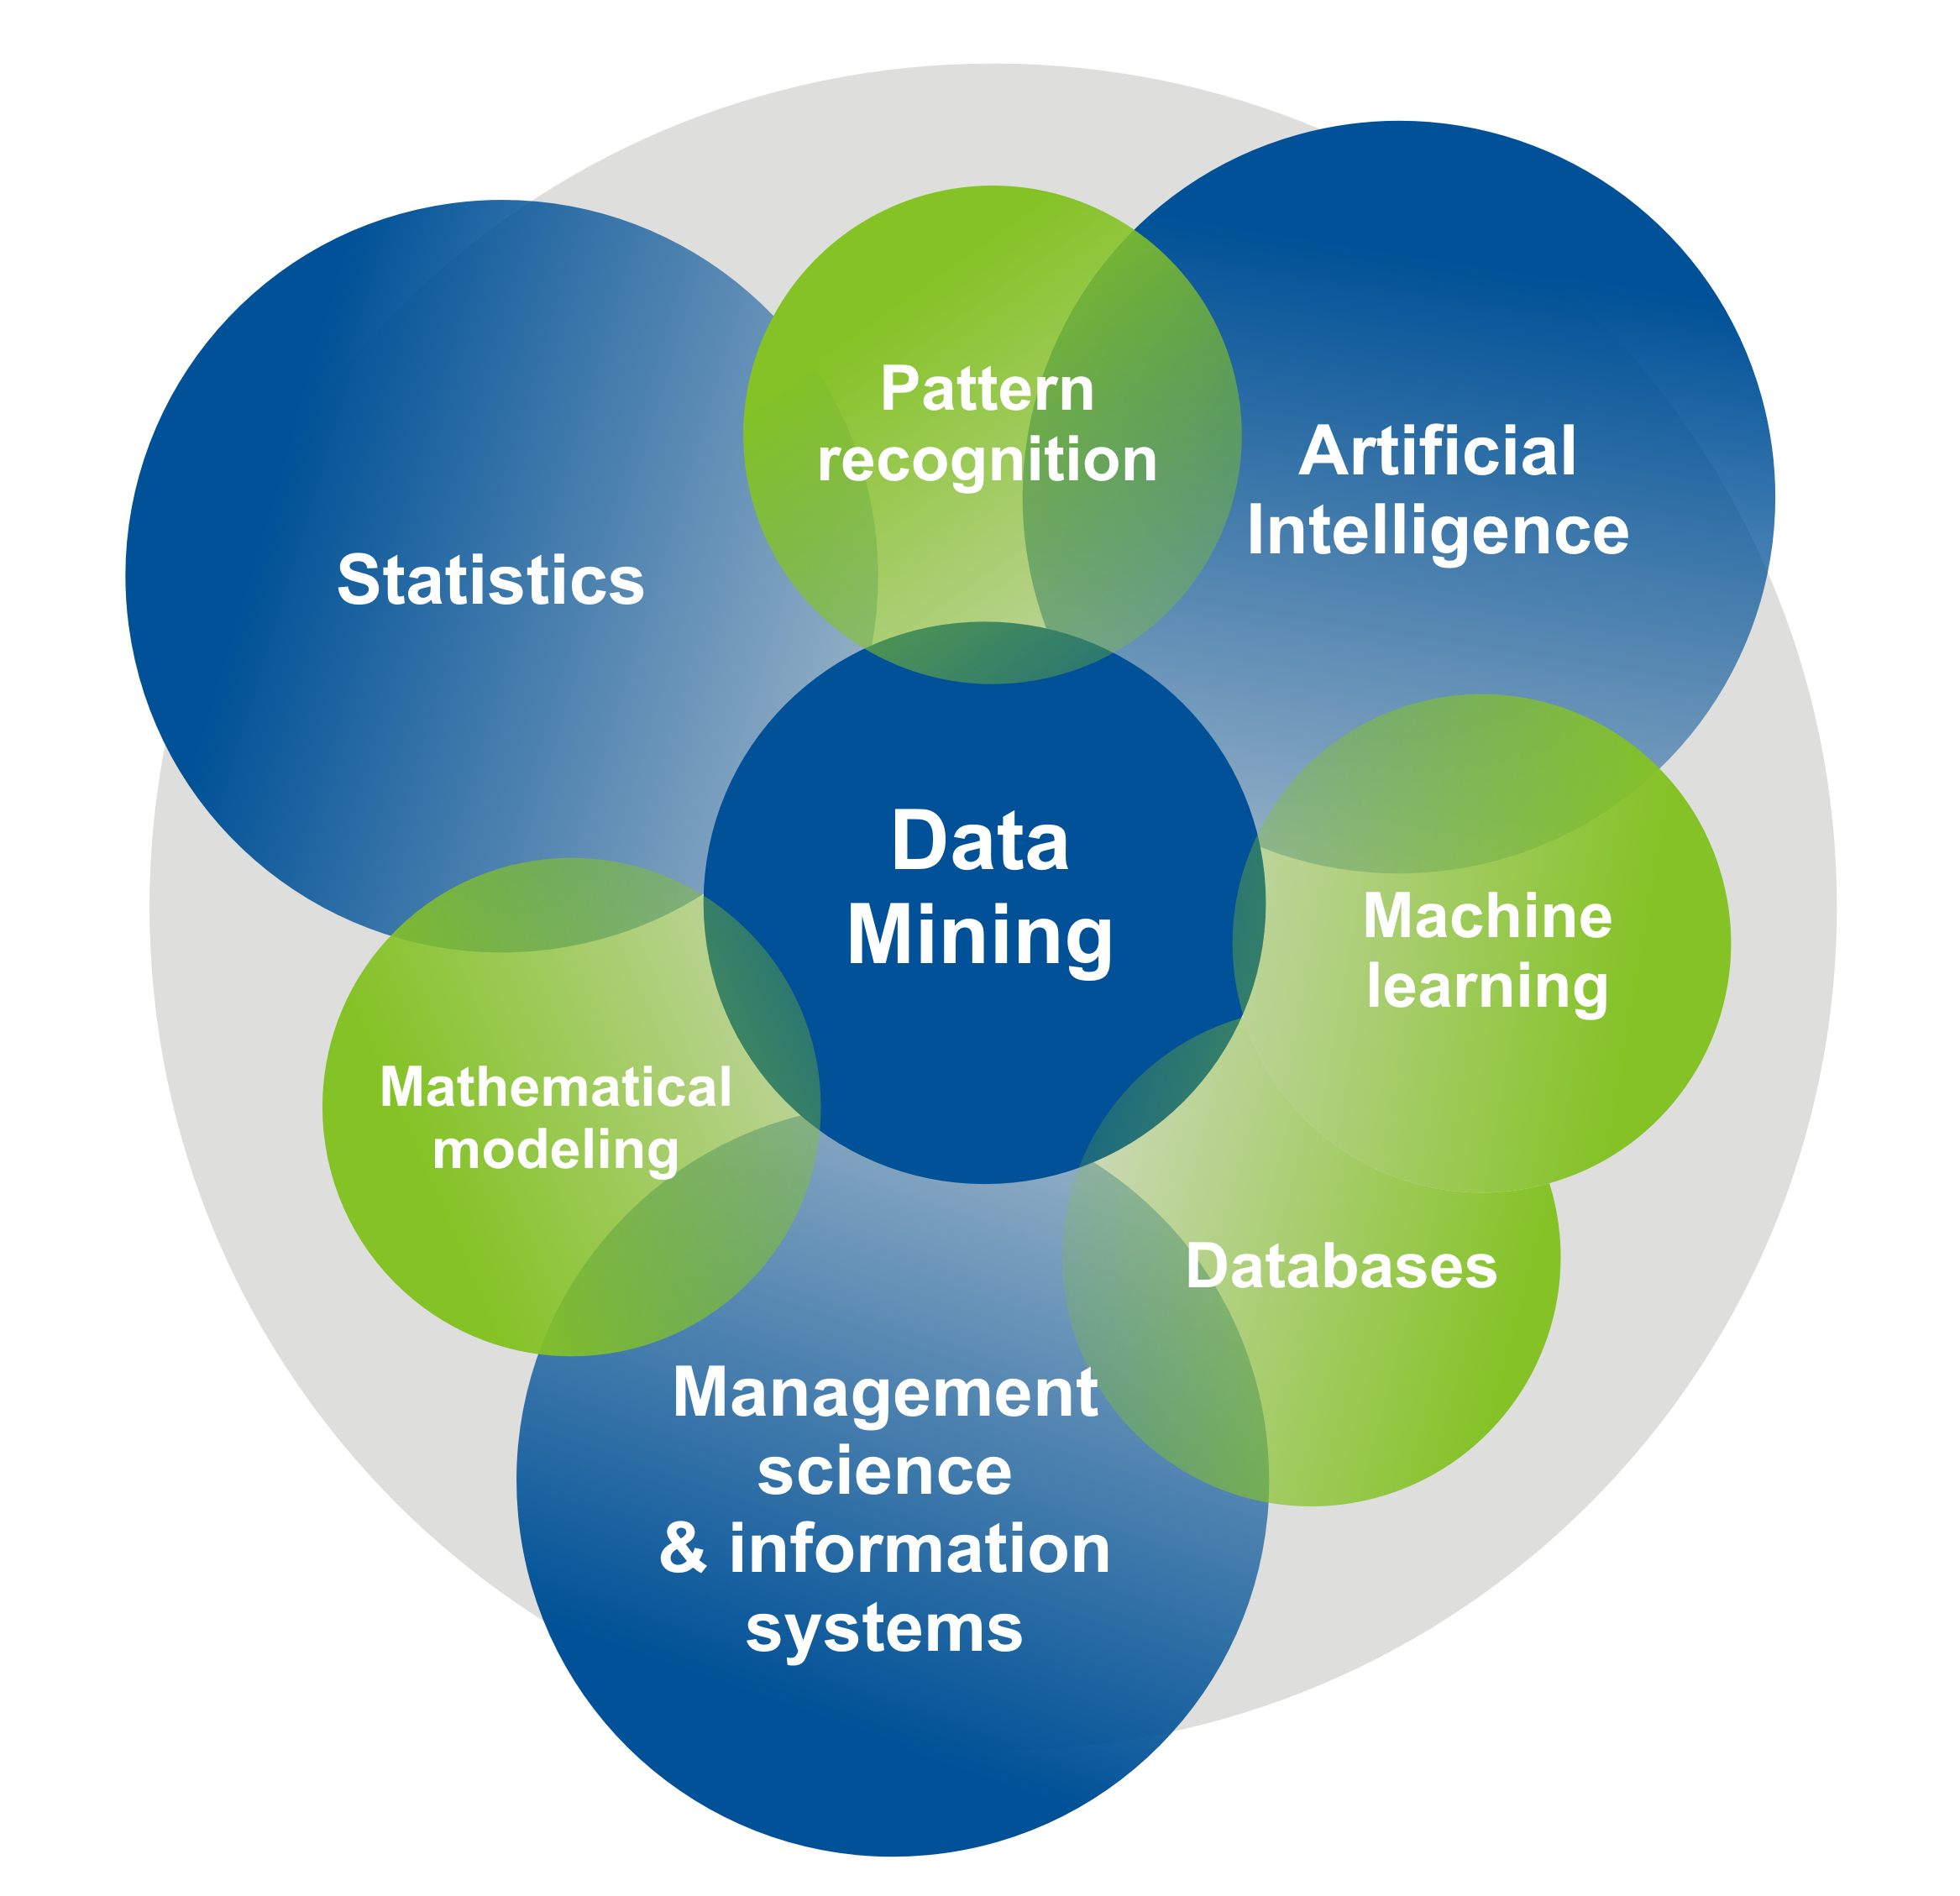
\includegraphics[scale=.3]{imagenes/data_mining.jpg}
	\caption{Componentes en la miner�a de datos}
	\label{intro1}
\end{figure}

Son tres las principales �reas que abarca la miner�a de datos: Estad�stica, Inteligencia Artificial y Manipulaci�n de sistemas de informaci�n, mientras que son distintos procesos los que interact�an entre estas ramas, tales como: Modelamiento Matem�tico, reconocimiento de patrones, Sistemas de almacenamiento persistente y machine learning.

Cada �rea en particular tiene un objetivo general y diversos objetivos espec�ficos. Sin embargo, estas �reas interact�an entre s�, con el fin de poder extraer patrones de informaci�n que generen conocimientos a partir de la data de procesada.

La miner�a de datos se utiliza en diferentes campos, tales como: Gen�tica, Evaluaciones prote�micas, Comercio, Sistemas de tr�nsito, Optimizaciones en procesos industriales, reconocimiento de patrones y rasgos cuantificables en enfermedades y m�s recientemente en �reas de din�micas moleculares y par�metros para la generaci�n de pipe lines automatizados de simulaciones cu�nticas en sistemas qu�micos.

El uso de la miner�a de datos y la b�squeda de patrones de comportamientos de datos de inter�s, no s�lo es un �rea que se enfoca en la investigaci�n. Diversas son las entidades privadas que ofrecen servicios de big data y data science, adem�s del sector p�blico, con el fin de detectar puntos cr�ticos de zonas de riesgo, zonas de accidentes, evaluaci�n o perfilaci�n de grupos de estudio, etc. 

\section{Problem�tica}

Actualmente, los sistemas de almacenamiento persistente, permiten disponer de informaci�n que es de inter�s para distintos tipos de entidades, las cuales depender�n del �rea a las que se dediquen. Sin embargo, cada �rea en particular, tiene objetivos similares, tales como:

\begin{itemize}
	
	\item Qu� significa los datos que tengo?
	\item Puedo personalizar y interpretar datos?
	\item Puedo optimizar procesos en base a la informaci�n que tengo sobre estos?
	\item Es factible aumentar la experiencia de usuario en cuanto a procesos de ventas y compras, personalizando sus �reas de cliente?
\end{itemize}

Son muchos los objetivos que se pueden encontrar y muchas las aplicaciones que implica esta t�cnica. No obstante, el hecho de tener data almacenada y no saber c�mo procesarla es un gran problema para muchas peque�as y medianas empresas, as� como para tambi�n ventas, laboratorios de investigaci�n, etc.

El deseo de aplicar miner�a de datos, con el fin de extraer informaci�n, es d�a a d�a, m�s frecuente. Sin embargo, un usuario com�n debe enfrentar la problem�tica de como afrontar el problema, adquirir las competencias, o simplemente, contratar servicios de data science, los cuales cobran altas sumas de dinero y emplean un tiempo elevado con el fin de llegar a una respuesta pronta.

Por otro lado, existen herramientas que facilitan la utilizaci�n de miner�a de datos, pero, el costo por conceptos de licencia es demasiado elevado y no permite abarcar diversas �reas y testear algoritmos variados. Mientras que por otro lado, existen m�dulos o librer�as que han sido implementadas en diversos lenguajes de programaci�n, con el fin de aplicar miner�as de datos, pero esto aumente a�n m�s la complejidad del tema, debido a que para implementar dicha labor, se requiere de conocimientos en programaci�n y en algunos casos, las implementaciones son engorrosas y requieren de un conjunto de arquitecturas que soporten dichas instancias.

Dado a lo anterior, es que se propone el desarrollo de una herramienta web, que permita la aplicaci�n de diversas t�cnicas de miner�a de datos y oriente de manera inteligente al usuario, esto implicar�a que no se requiere de un conocimiento de programaci�n, adem�s que las competencias en miner�a de datos deben ser m�nimas, puesto que la idea contempla la orientaci�n al usuario con respecto al objetivo que desea.

Durante este documento, se expone el dise�o de la herramienta, las metodolog�as a utilizar y los artefactos de software que se crear�n, con el fin de poder implementar esta herramienta en base a una metodolog�a de dise�o, adem�s se expone un resumen de las tecnolog�as actuales, cuales son las ventajas y desventajas que poseen cada una y en qu� se diferencia el software planteado con respecto a los existentes.

\subsection{Estado del Arte}

\section{Smart Training}

Smart Training es un sistema web, que facilita la utilizaci�n de t�cnicas de miner�a de datos, con el fin de evaluar caracter�sticas en set de datos, reconocer patrones, entrenar algoritmos de clasificaci�n, generar evaluaci�n de caracter�sticas, etc. Tiene por finalidad acercar la miner�a de datos a un p�blico que no posee las competencias para implementar modelos mediante utilizaci�n de m�dulos de programaci�n.

Smart Training se compone de 5 m�dulos, los cuales se detallan a continuaci�n.

\subsection{M�dulo de Procesamiento de Datos}

Este m�dulo tiene por objetivo cargar la data entregada en archivos de texto, eval�a los datos existentes, corrobora que no existan problemas, revisa el set de datos, encuentra valores nulos, codificaciones no permitidas, etc, a lo que, finalmente, entrega un resumen del proceso, exponiendo los resultados y de dicha tarea y comentando si es posible trabajar con dicho set cargado, en caso contrario, expone mensajes con recomendaciones a seguir.

\subsection{M�dulo de An�lisis Estad�stico}

Este m�dulo permite la evaluaci�n del set de datos contemplando, correlaciones, box plot, distribuciones mediante histogramas, scatter plot, gr�ficos de densidad de datos, adem�s de res�menes estad�sticos para cada atributo o caracter�stica en el set de datos que se est� trabajando.

\subsection{M�dulo de An�lisis de Features}

Este m�dulo permite evaluar las caracter�sticas en el set de datos y el aporte que �stas entregan, adicional a ello, contempla an�lisis mediante t�cnicas PCA, para generar reducciones de dimensionalidad, Mutual Information y t�cnicas basadas en correlaci�n, todas con el objetivo de explicar los comportamientos de �stas y c�mo influyen en el set de datos.

\subsection{M�dulo de Clustering}

Clustering es una de las t�cnicas m�s conocidas para asociar segmentos en una muestra, es decir, generar grupos o particiones que tengan un alto grado de diferencia entre ellas, pero cuyos integrantes en una partici�n dada, sean altamente similares.

Existen diferentes algoritmos de clustering y par�metros asociados a estos, los cuales tienen formas de encontrar particiones distintas, bas�ndose en distancias, medidas gausianas, generaci�n de hiper planos, etc.

Este m�dulo tiene por objetivo generar exploraci�n de dichas t�cnicas y algoritmos, con el fin de poder entregar particiones en el set de datos, adem�s, permite la evaluaci�n de dichas particiones con el fin de poder determinar si son estad�sticamente significativas o no, adem�s de cumplir con los criterios de similitud y diferenciaci�n mencionados previamente.

Normalmente, la b�squeda de particiones conlleva al hecho de generar modelos de clasificaci�n para nuevos ejemplos y determinar a qu� particiones se encuentran, o tambi�n, generar divisiones para implementar set de datos diferentes con comportamientos diferentes, de tal manera que a la hora de aplicar algoritmos de clasificaci�n, sus comportamientos presenten mayor eficiencia.

\subsection{M�dulo de Entrenamiento de Modelos}

Entrenar un modelo de clasificaci�n, predicci�n, implica tener un conjunto de elementos con su clasificaci�n o valor de predicci�n conocido, con el fin de poder, a partir de �ste, evaluar nuevos ejemplos, ya sea para clasificarlos o para predecir posibles valores de inter�s. Todas estas tareas, aplicando miner�a de datos, se logran mediante la implementaci�n de algoritmos de aprendizaje supervisado.

Existen diferentes algoritmos de aprendizaje supervisado, los cuales contemplan diferentes formulaciones matem�ticas y caracter�sticas, los cuales cumplen con dicha tarea, cada uno de estos, presenta caracter�sticas distintas, en relaci�n al funcionamiento del mismo, la elecci�n de un algoritmo por sobre otro, va de la mano con el hecho de las necesidades que el problema conlleva, ya sea, con el fin de entregar s�lo un resultado, adicionar valores que permitan explicar el porqu� de la clasificaci�n, etc. Normalmente, para un problema desconocido, es necesario implementar fases exploratorias que permitan evaluar diferentes algoritmos y sus par�metros. Con el fin de poder, a partir de dicha instancia y en base a m�tricas que permitan evaluar el desempe�o, seleccionar un algoritmo y sus par�metros.

Lo anterior, es el objetivo del m�dulo de entrenamiento de modelos, la idea de �ste, es recibir un set de datos con ejemplos clasificados o cuya respuesta tenga un valor conocido y aplicarle diversos algoritmos y variaciones de par�metros, entregando un resumen de las medidas de desempe�o obtenidas y efectuando un ranking seg�n medida, para que finalmente se pueda entregar una recomendaci�n de los mejores modelos para un cierto problema.

\subsection{Diagrama soluci�n}

\section{Objetivos y Alcances}

El objetivo general del proyecto contempla la implementaci�n de un sistema web denominado, \textit{Smart Training}, el cual permita la aplicaci�n de distintas t�cnicas de miner�a de datos a set de datos de inter�s del usuario, a partir de los cuales �ste pueda entender comportamientos de datos y generar conocimiento a partir de ellos.

Es importante destacar los objetivos espec�ficos que nacen dentro del desarrollo del proyecto.

\begin{enumerate}
	
	\item Dise�ar metodolog�a de software a utilizar.
	\item Comprender los requerimientos observados a partir del estado del arte.
	\item Evaluar las funcionalidades y atributos que tendr� el sistema.
	\item Comprender los usuarios y actores del software.
	\item Entender las secuencias y flujos de trabajo existentes en la herramienta.
	\item Crear modelos de conceptos, entidades y clases.
	\item Implementar los m�dulos propuestos.
	\item Implantar sistema.
\end{enumerate}

\section{Metodolog�a de Desarrollo de Software}

Existen diversas metodolog�as de desarrollo de software, las cuales contemplan diferentes caracter�sticas y se enfocan en distintos puntos objetivo. Algunos ejemplos son.

\begin{itemize}
	
	\item Metodolog�as �giles.
	\item Dise�o cascada.
	\item Dise�o estreslla.
	\item Iterativas.
\end{itemize}

Metodolog�a �gil, se utiliza cuando el objetivo se basa principalmente en sacar a producci�n el software de manera r�pida, no contempla procesos de dise�o complejos y simplemente se centra en el desarrollo del producto, lo cual permite, por un lado, poseer un producto en poco tiempo. Sin embargo, est� sometida a enmarcar errores debido a que no se consideraron patrones de dise�o.

El dise�o en cascada y tambi�n en estrella, se centran en los requerimientos de usuario y generar sub productos asociados al software final, los cuales cumplen un objetivo en particular del software, fueron muy utilizadas en los a�os 90, debido a la simplicidad que estos pose�an.No obstante, no contempla iteraciones para evaluar los flujos de trabajo, ni tampoco la utilizaci�n de paradigmas complejos de desarrollo de software.

Una de las metodolog�as m�s utilizadas, es la Iterativa, �sta contempla un conjunto de patrones de dise�o, los cuales est�n asociados a la evaluaci�n de las funcionalidades, los atributos, describir secuencias de flujos y asociar conceptos, es la metodolog�a que contempla un mayor conjunto de pasos. No obstante, es la que m�s asegura que a la hora de implementar, dicho proceso sea r�pido. El hecho de ser iterativa, implica que cada etapa entrega un artefacto de software, bajo el cual depende el siguiente, en nuevas etapas se hacen mejoras a los artefactos generados y se est� en constante feedback.

Adicional a las metodolog�as de software, existen diferentes paradigmas de programaci�n que son empleados en conjunto con dichas estrateg�as. Los dos principales son: Estructurado y Orientado a Objetos. En el primero, se sigue un orden secuencial del problema a desarrollar, no est� adaptado para grandes desarrollos, si no que m�s bien, es empleado en scripting y manejo de patrones en archivos de texto. Por otro lado, la programaci�n Orientada a Objetos (POO), cumple con la caracter�sticas de ser m�s cercana a la vida real, debido a que se basa en el dise�o de clases, que representan entidades las cuales pueden ser ficticias o reales. Presenta grandes ventajas debido a que posee las siguientes caracter�sticas.

\begin{itemize}
	
	\item \textit{Encapsulamiento}: Un Objeto es due�o de sus atributos y m�todos.
	\item \textit{Polimorfismo}: Un mismo m�todo, pueden tener significados diferentes para distintas clases.
	\item \textit{Reusabilidad}: Una clase modelada puede utilizarse en diversos proyectos debido a que siempre poseer� los mismos atributos y m�todos.
\end{itemize}

Adem�s de dichas caracter�sticas, la POO asocia conceptos abstractos a la programaci�n, tales como: herencia, dependencias, asociaciones y composiciones, las cuales aumentan m�s a�n, la usabilidad de este paradigma.

En esta ocasi�n, debido a la envergadura del proyecto, a las caracter�sticas que se espera que posea y a las ventajas que entregan las metodolog�as, se utilizar� el dise�o de software iterativo con objeto acoplado. Es decir, se dise�ar� teniendo en consideraci�n distintas iteraciones asociadas a los artefactos de software que se desarrollen, enfocando dicho dise�o a POO.
   %intro general al tema
\chapter{An�lisis}

La etapa de an�lisis del proyecto, contempla la evaluaci�n y determinaci�n de las diferentes funcionalidades que tendr� el sistema, asociado a los atributos que estos presentan y que permiten cuantificar de cierta manera el software. Tambi�n contempla las evaluaciones de los flujos asociados a cada funci�n y determina las secuencias de pasos a seguir para dar respuesta a cada una de �stas, exponi�ndolos en forma narrativa mediante los casos de uso. Finalmente se eval�an los conceptos existentes y que representan entidades dentro del software, los cuales forman parte del dise�o posterior.

\section{Funciones del Sistema}

\section{Atributos del Sistema}

\section{Actores y Usuarios}

\section{Casos de Uso}

\subsection{Diagramas de casos de uso}

\section{Diagramas de secuencia o colaboraci�n}

\section{Conceptos}

\subsection{Modelo Conceptual}

\section{Entidades}

\subsection{Modelo de Entidades}
 %hipotesis
\chapter{Dise�o}

\section{Arquitectura de Software}

\section{Diagramas de Interacci�n}

\section{Diagrama de Clases}

\section{Diagramas de Estado}

 %objetivos
\chapter{Planificaci�n}

\section{Etapas del Proyecto}

 %metodologias y desarrollos de modelos
\begin{thebibliography}{X}

\bibitem{intro1} \textit{Data Mining Curriculum}. ACM SIGKDD. 2006-04-30. Retrieved 2014-01-27.

\bibitem{intro2} Clifton, Christopher (2010). \textit{Encyclopedia Britannica: Definition of Data Mining}. Retrieved 2010-12-09.

\bibitem{intro3} Hastie, Trevor; Tibshirani, Robert; Friedman, Jerome (2009). \textit{The Elements of Statistical Learning: Data Mining, Inference, and Prediction}. Retrieved 2012-08-07.

\bibitem{intro4} Fayyad, Usama; Piatetsky-Shapiro, Gregory; Smyth, Padhraic (1996). \textit{From Data Mining to Knowledge Discovery in Databases} (PDF). Retrieved 17 December 2008.

\end{thebibliography}
%%% ambiente glosario
%\begin{glosario}
%  \item[El primer t�rmino:] Este es el significado del primer t�rmino, realmente no se bien lo que significa pero podr�a haberlo averiguado si hubiese tenido un poco mas de tiempo.
%  \item[El segundo t�rmino:] Este si se lo que significa pero me da lata escribirlo...
%\end{glosario}


%% genera las referencias
%\nocite{*}
%\bibliography{bib/b1}

%% comienzo de la parte de anexos


%% contenido del primer anexo
%% fin
\end{document}

   
